\documentclass[12pt,a4paper]{article}
\usepackage[left=2cm,right=2cm,top=2cm,bottom=2cm]{geometry}
\usepackage[utf8]{inputenc}
\usepackage[T2A]{fontenc}
\usepackage{amsmath}
\usepackage{amssymb}
\usepackage{graphicx}
\usepackage[russian]{babel}
\usepackage{indentfirst}
\usepackage{listings}
\usepackage{xcolor}
\usepackage{hyperref}

\hypersetup{
  colorlinks=true,
  urlcolor= blue,
  citecolor=blue,
  linkcolor= blue,
}

\title{Отчет по лабораторным работам №3-4 по дисциплине "Математическая статистика"}
\author{Скворцов Владимир Сергеевич (5030102/10201)}
\date{\today}

\begin{document}

	\begin{titlepage}

		\Large

		\begin{center}
			Санкт-Петербургский \\ Политехнический университет Петра Великого

			\vspace{10em}

			\textbf{Отчет по лабораторным работам №3-4} \\
			\textbf{по дисциплине}\\
			"\textbf{Математическая статистика}"

			\vspace{2em}

		\end{center}

		\vspace{6em}

		\newbox{\lbox}
		\savebox{\lbox}{\hbox{Скворцов Владимир Сергеевич}}
		\newlength{\maxl}
		\setlength{\maxl}{\wd\lbox}
		\hfill\parbox{12cm}{
			\hspace*{3cm}\hspace*{-5cm}Студент:\hfill\hbox to\maxl{Скворцов Владимир Сергеевич\hfill}\\
			\hspace*{3cm}\hspace*{-5cm}Преподаватель:\hfill\hbox to\maxl{Баженов Александр Николаевич}\\
			\\
			\hspace*{3cm}\hspace*{-5cm}Группа:\hfill\hbox to\maxl{5030102/10201}\\
		}

		\vspace{\fill}

		\begin{center}
			Санкт-Петербург \\ 2024
		\end{center}

	\end{titlepage}

	\tableofcontents\newpage

	\section{Постановка задачи}
	\subsection{Описательная статистика}
	Для 5 распределений:\\
	\begin{itemize}
		\item Нормальное распределение $N(x, 0, 1)$
		\item распределение Коши $C(x, 0, 1)$
		\item Распределение Стьюдента $t(x, 0, 3)$ с тремя степенями свободы
		\item Распределение Пуассона $P(k, 10)$
		\item Равномерное распределение $U(x, -\sqrt3, \sqrt3)$
	\end{itemize}

	Сгенерировать выборки размером 20 и 100 элементов.\\
	Построить на одном рисунке бокс-плот Тьюки.

	\section{Теоретическое обоснование}

	\subsection{Функции распределения}

	\begin{itemize}
		\item Нормальное распределение

		\begin{equation} \label{eq:normal}
			N(x, 0, 1) = \frac{1}{\sqrt{2\pi}}e^\frac{-x^2}{2}
		\end{equation}

		\item Распределение Коши

		\begin{equation} \label{eq:cauchy}
			C(x, 0, 1) = \frac{1}{\pi}\frac{1}{x^2+1}
		\end{equation}

		\item Распределение Стьюдента $t(x, 0, 3)$ с тремя степенями свободы

		\begin{equation} \label{eq:student}
			t(x, 0, 3) = \frac{6\sqrt3}{\pi(3 + t^2)^2}
		\end{equation}

		\item Распределение Пуассона

		\begin{equation} \label{eq:poisson}
			P(k, 10) = \frac{10^k}{k!}e^{-10}
		\end{equation}

		\item Равномерное распределение

		\begin{equation} \label{eq:uniform}
			U(x, -\sqrt3, \sqrt3) = \begin{cases}
				\frac{1}{2\sqrt3} & \mbox{при} \; |x| \leq \sqrt3\\
				0 & \mbox{при} \; |x| > \sqrt3
			\end{cases}
		\end{equation}
	\end{itemize}

	\subsection{Бокс-плот Тьюки}

	Боксплот (англ. box plot) — график, использующихся в описательной статистике, компактно изобрадающий одномерное распределение вероятностей. Такой вид диаграммы в удобной форме показывает медиану, нижний и верхний квартили и выбросы. Границами ящика служат первый и третий квартили, линия в середине ящика — медиана. Концы усов — края статистически значимой выборки (без выброса). Длину <<усов>> определяют разность первого квартиля и полутора межквартальных расстояний и сумма третьего квартиля и полутора межквартальных расстояний. Формула имеет вид

	\begin{equation} \label{eq:box_plot}
		X_1 = Q_1 - \frac{3}{2}(Q_3 - Q_1), \ X_2 = Q_3 + \frac{3}{2}(Q_3 - Q_1),
	\end{equation}

	где $X_1$ — нижняя граница уса, $X_2$ — верхняя граница уса, $Q_1$ — первый квартиль, $Q_3$ - третий квартиль.
	Данные, выходящие за границы усов (выбросы), отображаются на графике в виде маленьких кружков.
	Выбросами считаются величины $х$, такие что:

	\begin{equation} \label{eq:outlier}
		\left[
			\begin{array}{ll}
					x < X_1^T \\
					x > X_2^T
			\end{array}
		\right .
	\end{equation}

	\section{Описание работы}
	Лабораторные работы выполнены с использованием Python и его сторонних библиотек \verb!numpy!, \verb!pandas!, \verb!matplotlib!, \verb!seaborn! были построены гистограммы распределений и посчитаны характеристики пложения.

	Ссылка на GitHub репозиторий: \href{https://github.com/vladimir-skvortsov/spbstu-mathematical-statistics}{https://github.com/vladimir-skvortsov/spbstu-mathematical-statistics}

	\newpage

	\section{Результаты}

	\subsection{Гистограммы и графики плотности распределения}

	\begin{figure}[htbp!]
		\begin{center}
			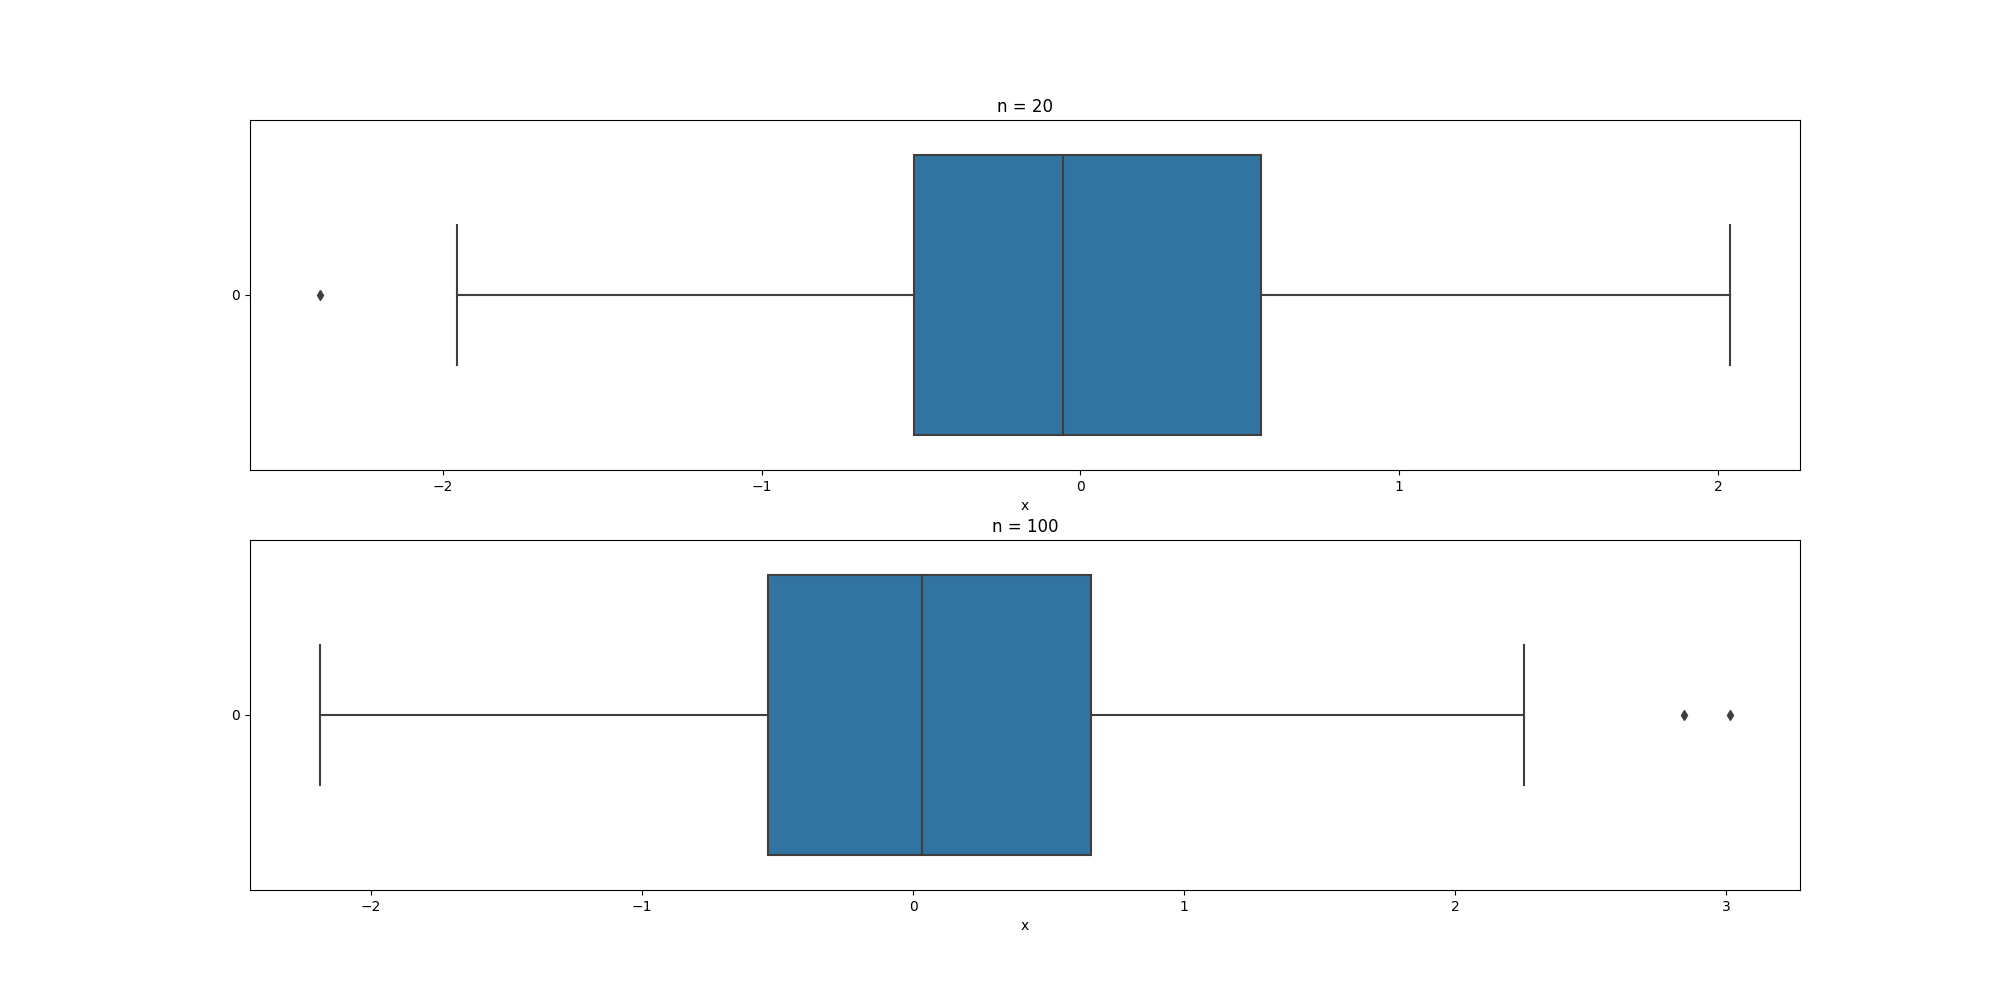
\includegraphics[width = 1.12\linewidth]{graphics/normal.png}
			\caption{Нормальное распределение \ \eqref{eq:normal}}
		\end{center}
	\end{figure}

	\begin{figure}[htbp!]
		\begin{center}
			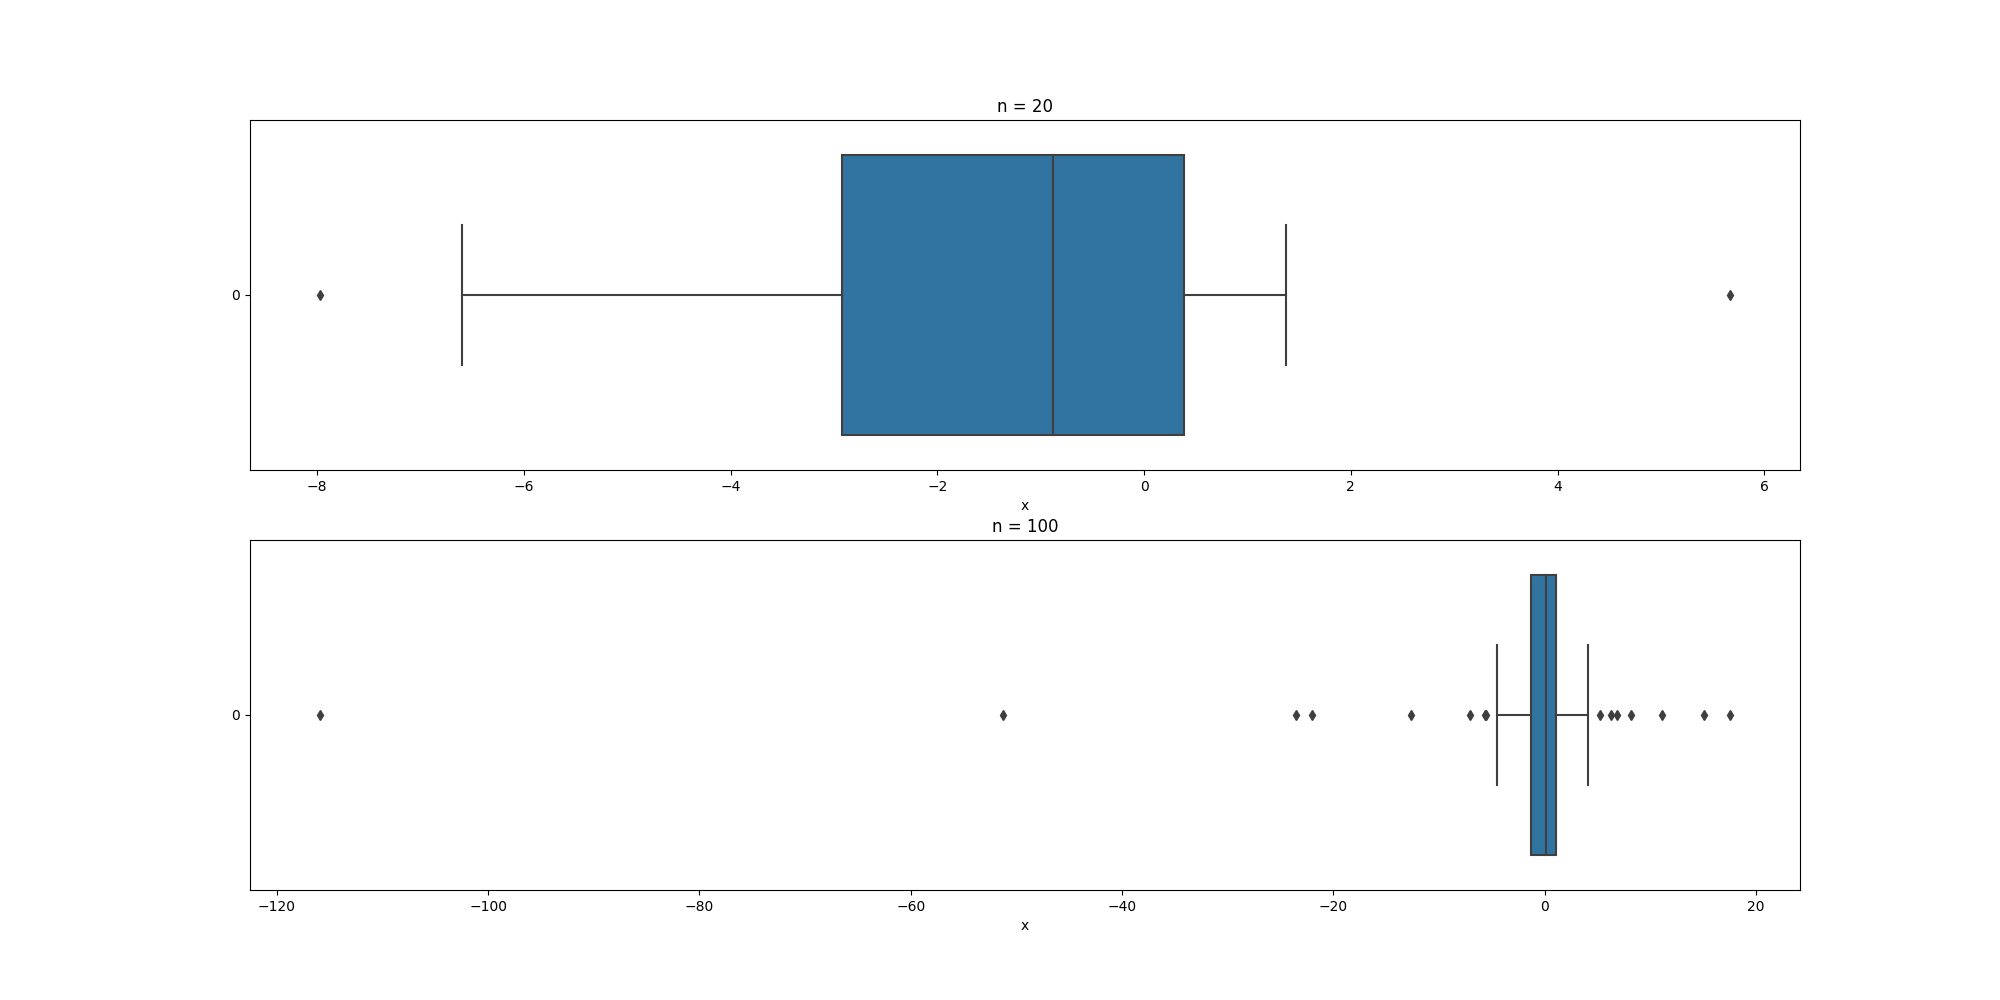
\includegraphics[width = 1.12\linewidth]{graphics/cauchy.png}
			\caption{Распределение Коши \ \eqref{eq:cauchy}}
		\end{center}
	\end{figure}

	\newpage

	\begin{figure}[htbp!]
		\begin{center}
			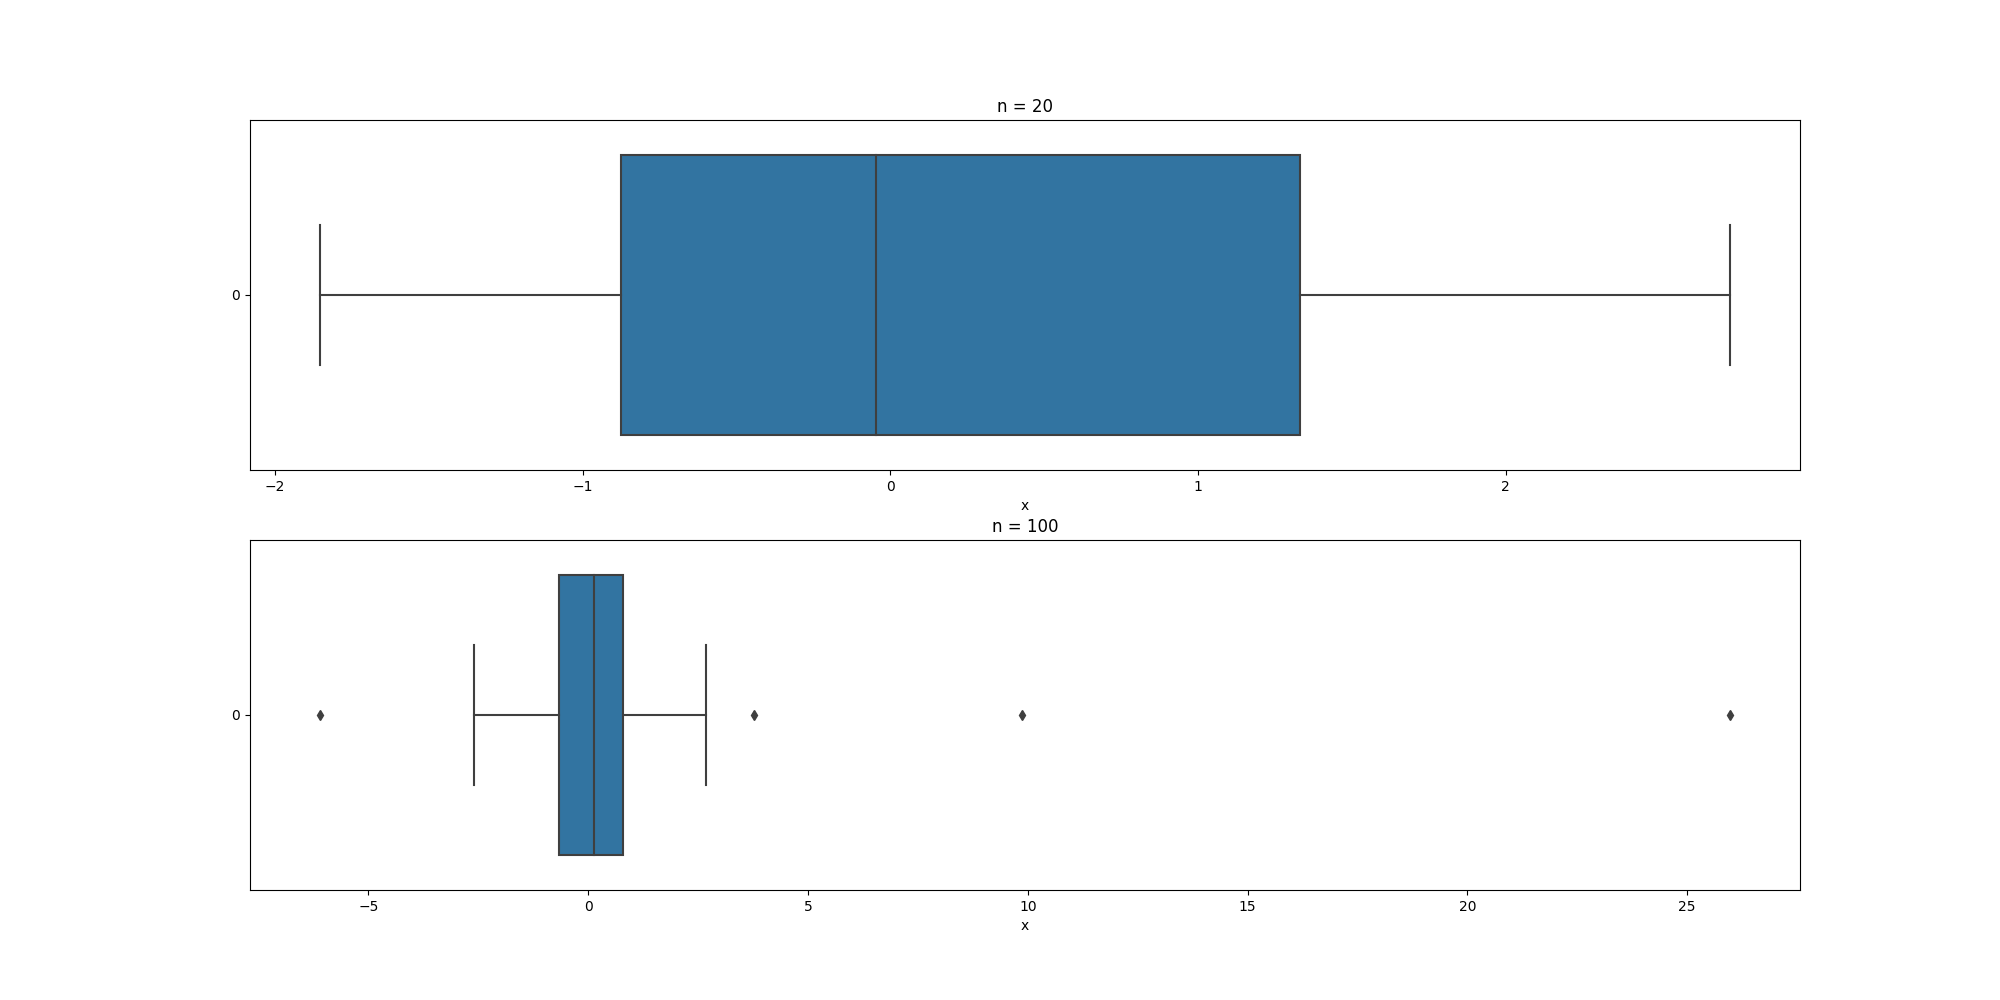
\includegraphics[width = 1.12\linewidth]{graphics/student.png}
			\caption{Распределение Стьюдента \ \eqref{eq:student}}
		\end{center}
	\end{figure}

	\begin{figure}[htbp!]
		\begin{center}
			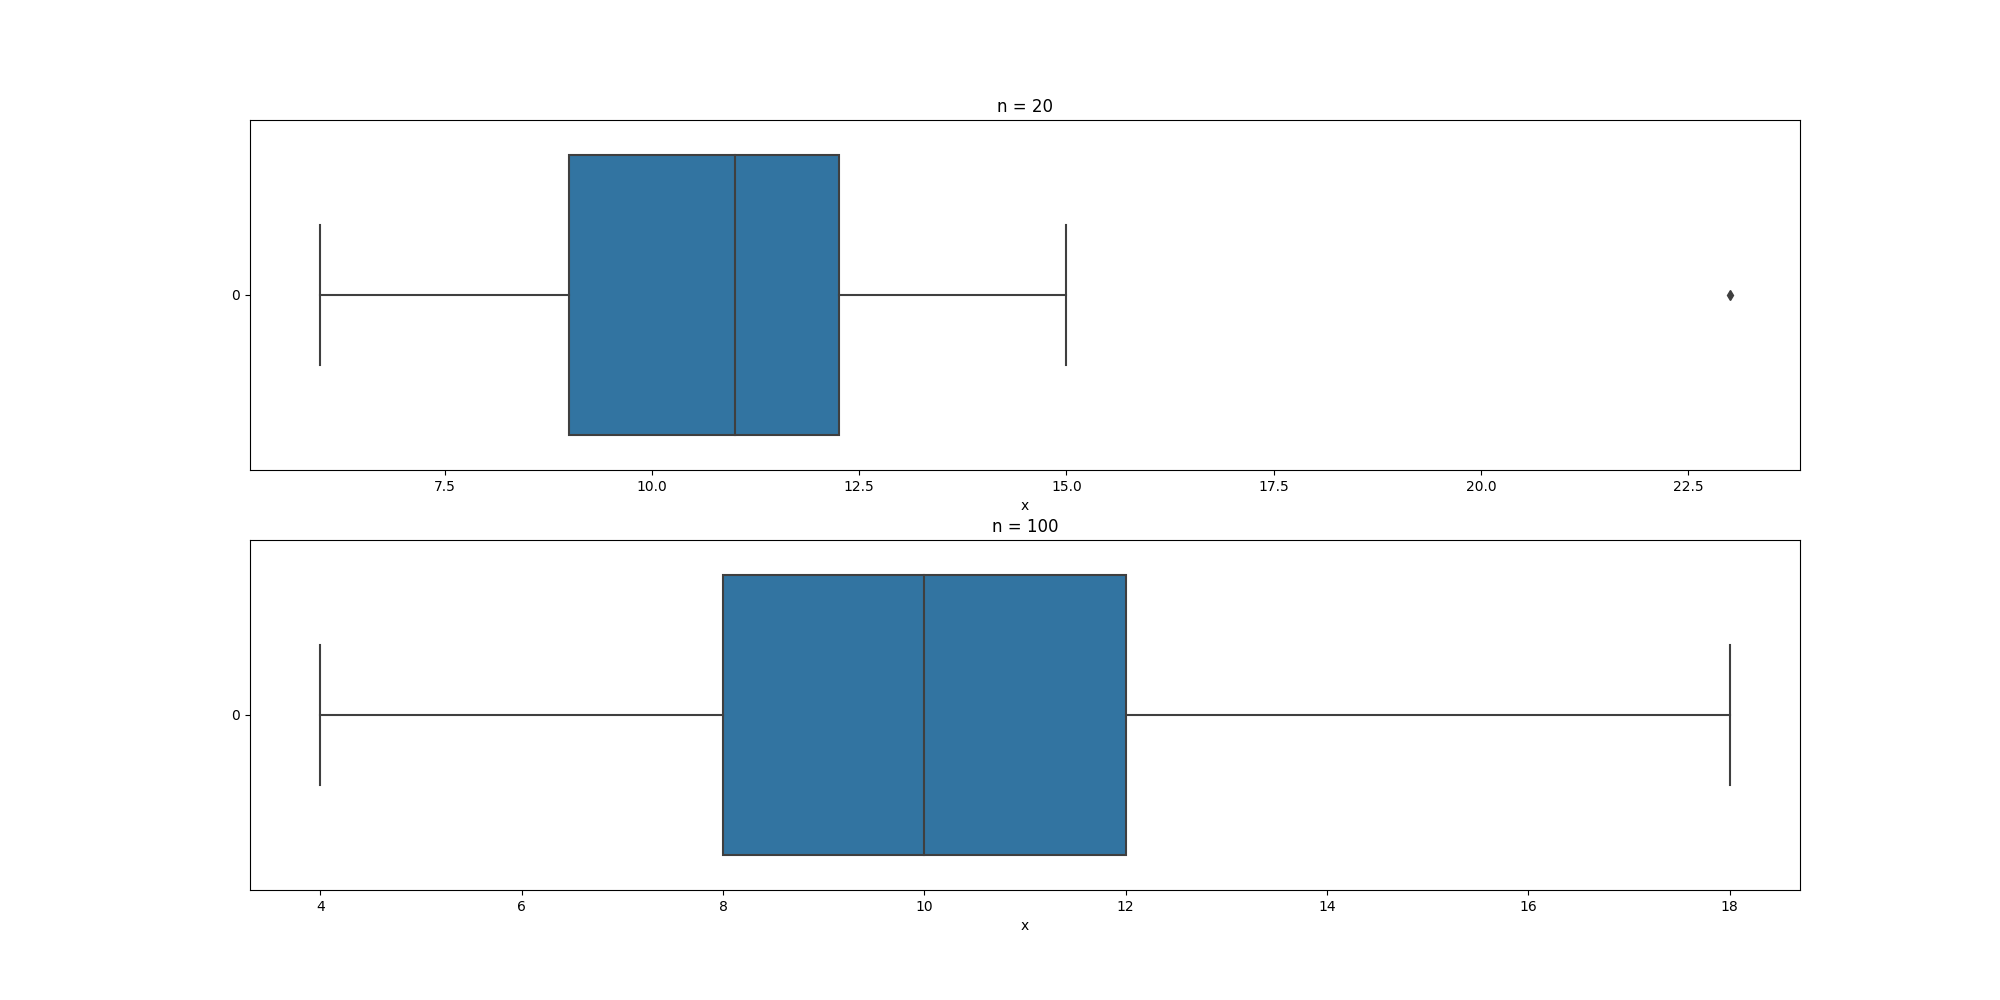
\includegraphics[width = 1.12\linewidth]{graphics/poisson.png}
			\caption{Распределение Пуассона \ \eqref{eq:poisson}}
		\end{center}
	\end{figure}

	\begin{figure}[htbp!]
		\begin{center}
			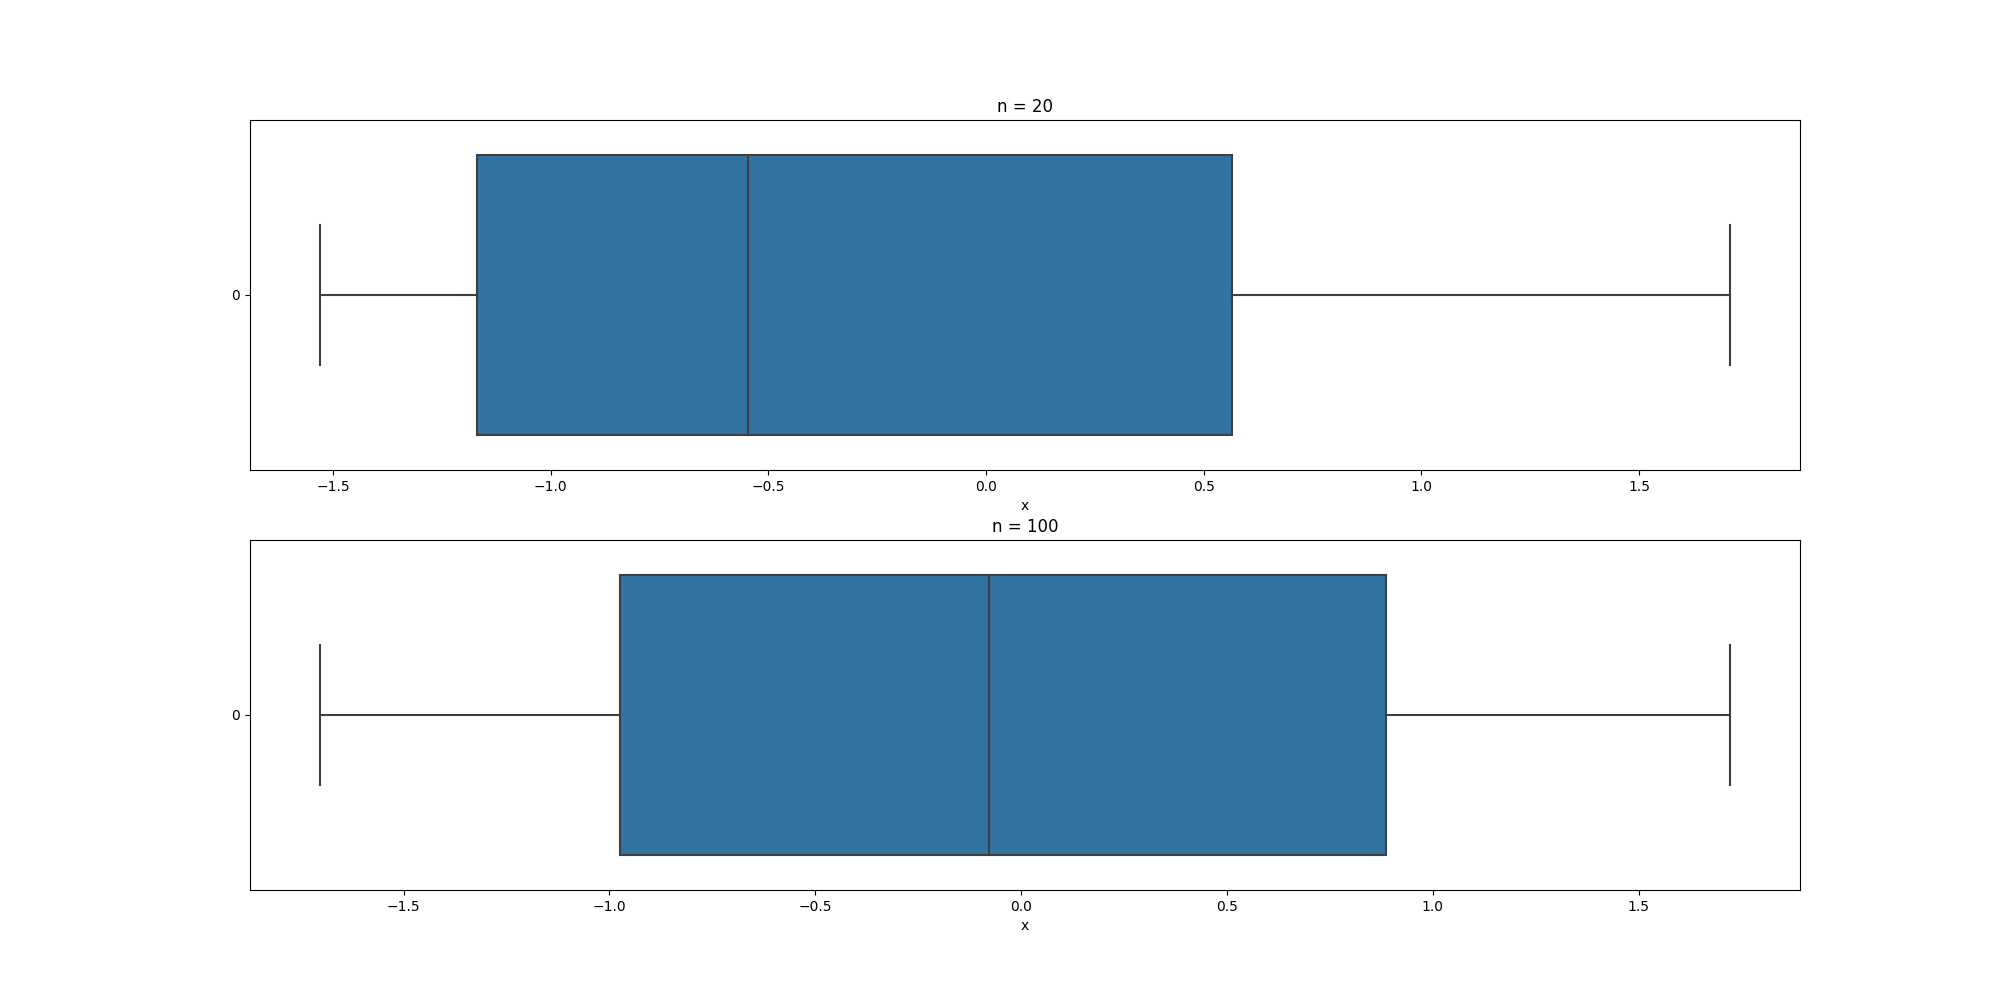
\includegraphics[width = 1.12\linewidth]{graphics/uniform.png}
			\caption{Равномерное распределение \ \eqref{eq:uniform}}
		\end{center}
	\end{figure}

	\newpage

	\section{Выводы}

	В процессе выполнения лабораторной работы был проведен анализ пяти уникальных распределений: нормальное, Коши, Стьюдента, Пуассона и равномерное.
	Были сгенерированы выборки разных объемов для каждого из них - 10, 50 и 1000 элементов.
	Были созданы гистограммы каждого распределения и нанесены на них графики плотности соответствующих распределений, что облегчило наглядное сопоставление формы распределения выборок с их теоретическими аналогами.
	Были также рассчитаны разные показатели положения и рассеяния для каждой выборки, включая выборочную среднюю величину, медиану, полусумму крайних элементов выборки, полусумму квартилей и усеченное среднее.
	Использовалась стандартная формула для оценки дисперсии. \\

	На основании полученных данных были сделаны следующие выводы:

	\begin{enumerate}
		\item В случае нормального распределения, оценки показателей положения и рассеяния становятся ближе к их теоретическим значениям по мере увеличения размера выборки.
		\item Для распределения Коши показатели положения и рассеяния менее стабильны и могут сильно отличаться от теоретических даже при больших размерах выборки.
		\item Распределение Стьюдента при небольших размерах выборки также демонстрирует определенную нестабильность оценок, однако с увеличением размера выборки результаты становятся более точными.
		\item Для распределения Пуассона и равномерного распределения, оценки показателей положения и рассеяния кажутся стабильными при любом объеме выборки.
		\item В общем, выборочное среднее является наиболее чувствительным к экстремальным значениям по сравнению с медианой, особенно в меньших выборках. Однако с увеличением размера выборки, влияние этих экстремальных значений на среднее значение уменьшается. В то же время, медиана обычно более устойчива к выбросам и мало варьирует с изменением размера выборки.
		\item Медиана является чувствительной к типу распределения: в нормальном и распределении Стьюдента медиана равна среднему, в распределении Коши она дает надежные, устойчивые к выбросам оценки, в Пуассоновском приближается к среднему, и в равномерном равна половине суммы минимального и максимального значений.
	\end{enumerate}
\end{document}
